% 9/12/13  (started from scratch)


\hspace{0.5cm}



\section{Comparison of Data and Simulation}
\label{compDataSim}

%\textbf{\textcolor{red}{Comment: Think about having a separate section on our encounters and dealings of various issues regarding simulation.}}
%Suppose, $n^{+}$ and $n^{-}$ are the faraday cup normalized counts in a given \wq bin for helicity 1 (+) and helicity 0 (-) states. Then the statistical error in the polarized count difference $\Delta n^{-}$ is given by $\sqrt{n^{+}+n^{-}}$\footnote{\textbf{\textcolor{red}{Comment: This footnote may be moved to another place/section (eg. data grouping) later on:}} There are different data sets (run numbers) based on whether half-wave-plate (HWP) was inserted or not, and whether the target polarization was in parallel or anti-parallel directions. So, a careful investigations and organizing of the run numbers into different groups were done where each group had the same HWP and target polarization states and nearly stable total Fcup normalized counts. And, for each of these subgroups, the histograms of the polarized counts were made first separately and at the time of \gone extraction, they were combined into one by making sure the total area under the quasi-elastic peaks would have the same sign in each data subsets, which means if the W histogram from any of the data subsets happened to have the elastic peak going negative, we would rescale the histogram with a factor of ``-1'' to invert the whole thing before combining with the other histograms from the other data subsets.}. % This part done in getNcombineClasHistosFrmGrpOp.C

Using our final values for the smear parameters, the simulated data were passed through GPP and then reconstructed with RECSIS. 
 Finally, all applicable cuts %\footnote{Initially, we started out from different cuts, especially those on EC-sampling fraction, vertex-Z and the fiducial cuts. But, to solve the various simulation issues and the discrepancies in the comparison between the data and simulation, they were modified and we arrived at the current set of cuts as listed in section \ref{allCuts}}
  and corrections were applied to both sets of polarized simulation data. Because the CC was turned off in GSIM for the simulation, 
 all experimental data cuts except those depending on CC were %all the cuts applied on experimental data (except those depending on CC) were also 
  applied to the simulated data. However, the cuts were modified (see Sec. \ref{allCuts}) to account for differences between simulation and data.
%There are some important details on how to handle detectors (like the CC and, to a lesser extent, the EC) which are known to be imperfectly simulated in GSIM (if at all), and how to correct for further inefficiencies (for instance luminosity-dependent tracking inefficiencies) - the simulated data have to be corrected for those ``by hand''. The details will be described elsewhere. We also have to account for pions and other background mis-identified as electrons and for electrons from pair-symmetric decays that are present in the data (as part of the term $Bg$ in Eq.~\ref{Delndef}) but not in the simulation. Finally, we have to account for the polarized background by adjusting the simulated  or experimental data appropriately (see Section~\ref{Bg}).

In the end, we had two sets of simulated events (for the two cases of $\Delta \sigma \geq 0 $ and $\Delta \sigma < 0$) in each kinematic bin. The number of these two type of events in each bin were then cross-normalized with respect to each other by their respective cross-section map integrals and the number of %thrown/generated
generated Monte-Carlo events and then combined to make the simulated polarized count difference $\Delta n$. To do that, the number of simulated event counts in a kinematic bin corresponding to the positive $\Delta \sigma$ %polarization 
was kept unchanged but the one corresponding to the negative $\Delta \sigma$ %polarization 
was multiplied with the following normalization factor:

\begin{equation}
 norm^- = \frac{\sigma^-_{tot}}{\sigma^+_{tot}}\times \frac{N^+}{N^-}
\end{equation}
where $\sigma^{+/-}_{tot}$ and $N^{+/-}$ are the total integral %area 
of the cross section map and the corresponding number of Monte-Carlo events generated for each of the polarization cases (+/-).
 %scalePPvNP=(xsMapTotNegPol/xsMapTotPosPol)*(pFlNum*1.0/nFlNum);  in GetNormalizeSimXsDiffHistos(..) of extractStrFnG1.C




The next step was to properly cross-normalize the simulated events to the data. %, as outlined in the introduction.
For this, we %simply 
found the scale factor $SF$ necessary to have the same $\Delta n$ in the quasi-elastic region (e.g., $0.9 \le W \le 1.0$). This factor represents the ratio

\begin{equation}
 SF = \frac{n^+ - n^-}{\Delta n(simul)} % = \frac{{\mathcal L}_r  \cdot P_b P_t }{{\mathcal L}_s}
\end{equation}
%since we assume that the simulation for the cross section difference in this region is reliable % ``perfect''
since the physics of QE is known (from form factors etc), we expect the simulation in this region is reliable %xz
 and all other factors\footnote{The scaling factor (SF) accounts for the luminosity, the product of the beam and target polarization ($P_bP_t$, and all other constant efficiency factors such as dead time, overall trigger efficiency, average tracking efficiency etc.} are common to the simulation and the data.
 In fact, we chose one \qsqs bin (the $20^{th}$ one - for which the agreement between the data and simulation was among the best) and calculated above ratio to get the global preliminary value of the scaling factor $SF_{20}$. The simulated $\Delta n$ was then multiplied with this factor to get our best ``prediction'' of the real data in all the kinematic bins, in order to directly compare it with the real data (see Figs. \ref{xsComp7} and \ref{xsComp8}). 




\begin{figure}[H] %ht, htpb (p - float, b = bottom, h=? t = top)
%  \leavevmode 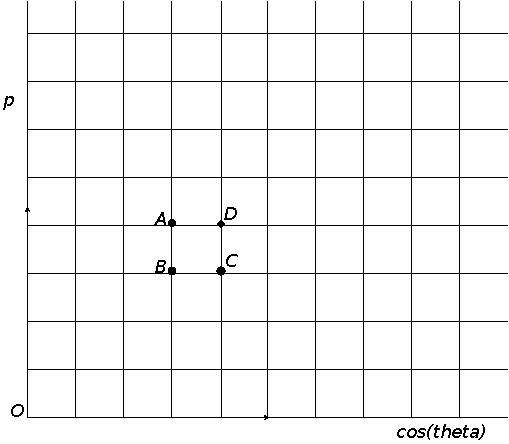
\includegraphics[width=0.6\textwidth]{chap4simul/Figures/kineGrid_steg.jpg} 
  %\leavevmode 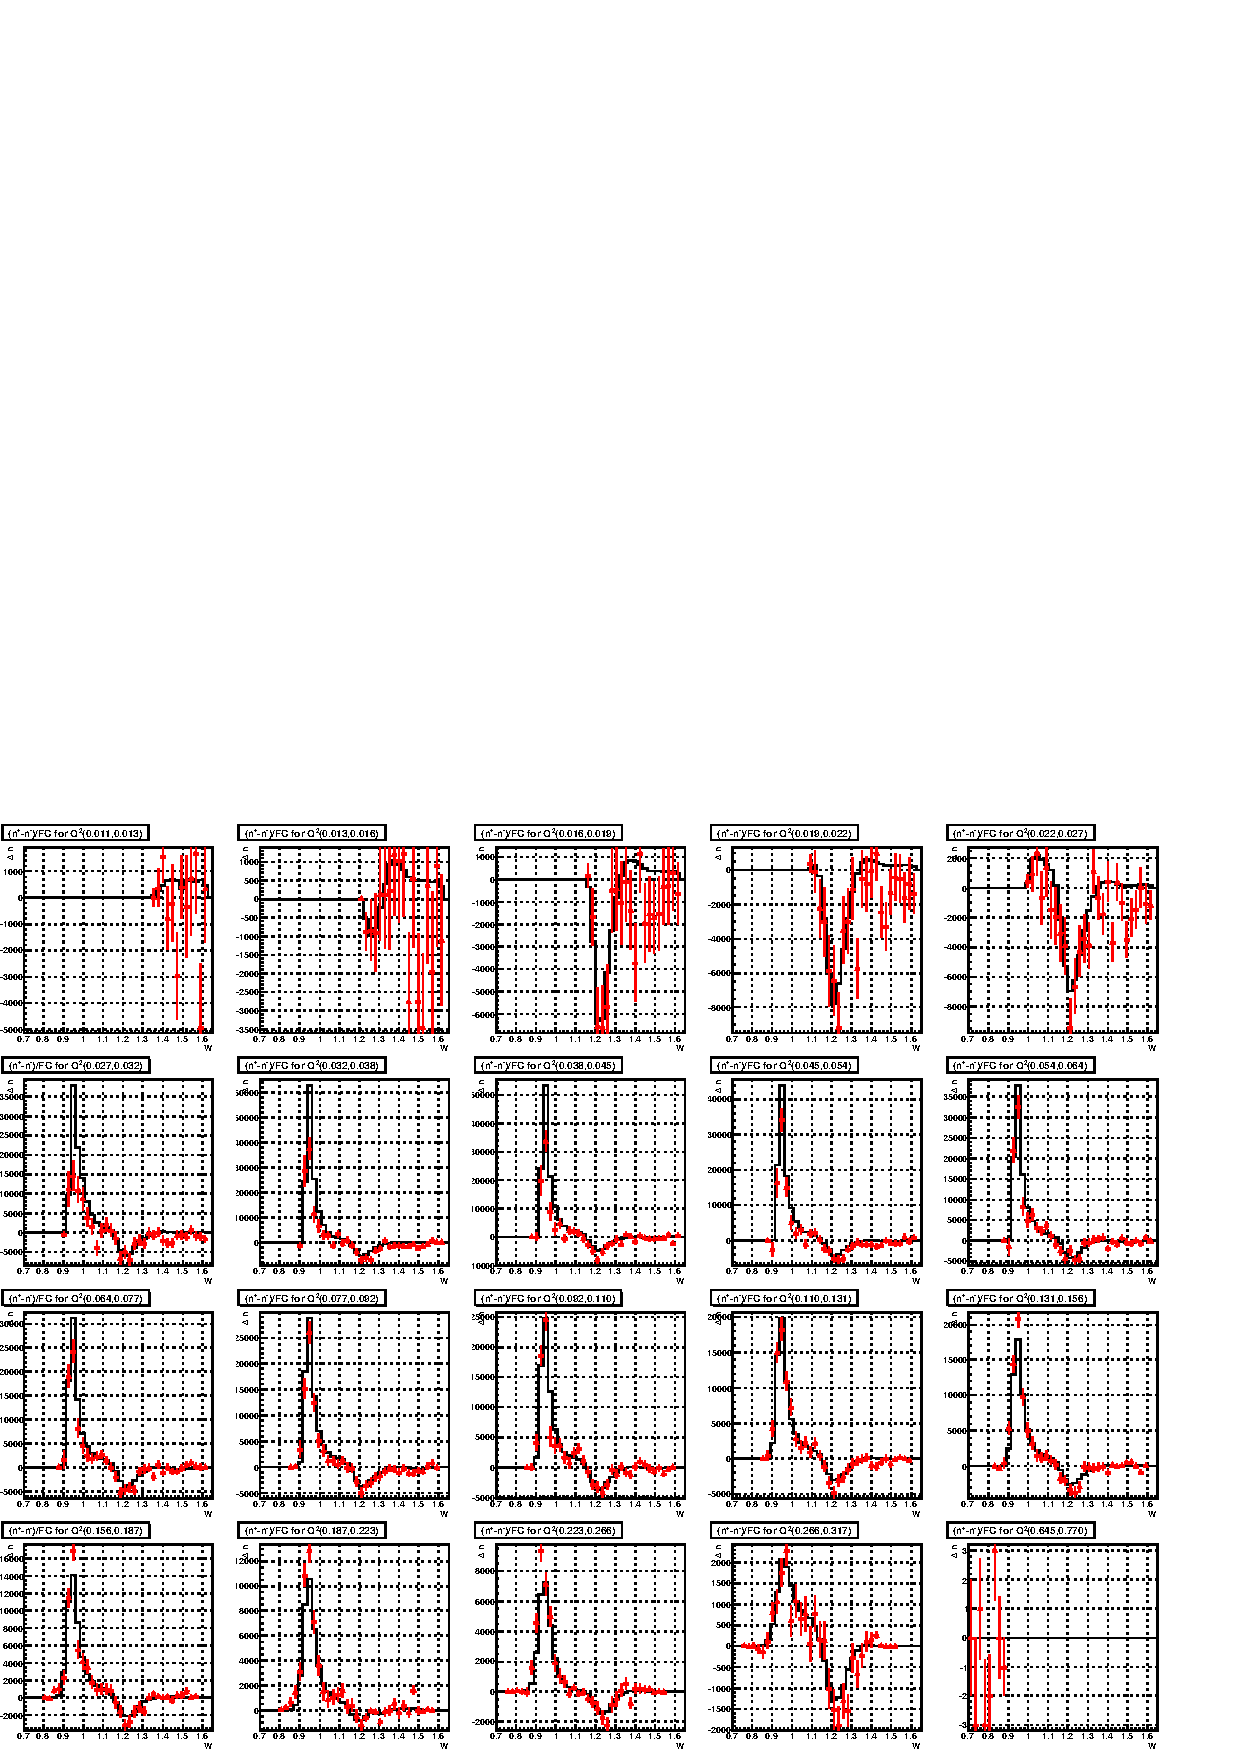
\includegraphics[width=1.0\textwidth]{figuresEG4/FigAnal/xsDifEb7VzD57HistC194S139.png}
  %  \caption[$\Delta n$ for data and simulation]{Comparison of polarized count differences from 1.3 GeV experimental (red points with error bars) and simulation data (black histograms). %\textbf{\textcolor{red}{I plan to change plots like these by throwing out the first and last very low or no statistics bins ..}} 
  %\leavevmode 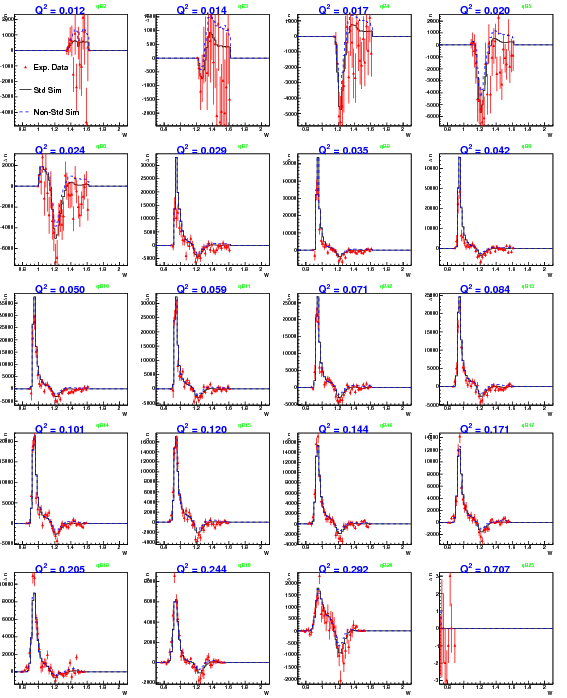
\includegraphics[width=1.0\textwidth]{figuresEG4/FigAnal/xsDiff_StdD57_nStdD68C194S139Eb7Wbins70N.png} 
  \leavevmode 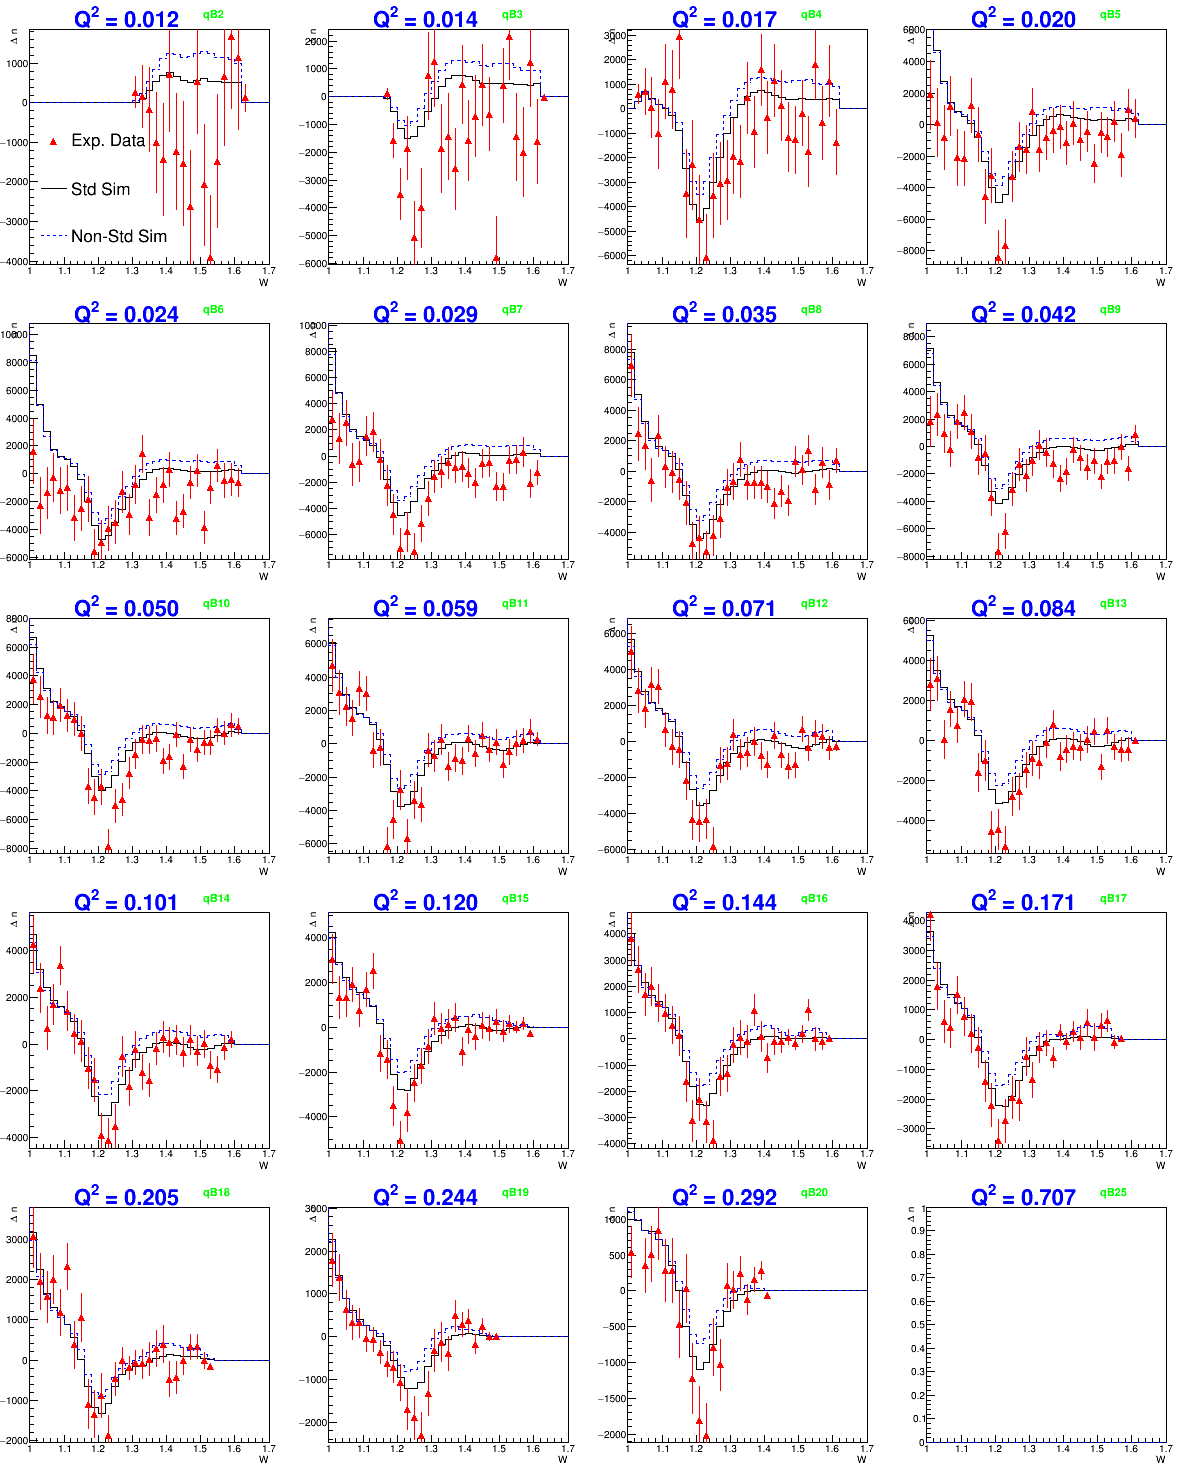
\includegraphics[width=0.97\textwidth]{figuresEG4/FigAnal/xsDiff_StdD79_nStdD80C71S181Eb7Wbins70NZmd.png}
  \caption[$\Delta n$ for data and simulation]{Comparison (in different \qsqs bins) of polarized count differences from 1.3 GeV experimental (red points with error bars) and two versions of normalized simulation data. The black continuous histograms are for ``standard'' simulation with values of $A_1$ in the inelastic region as given by the model used in the simulation. The blue dotted histograms are for ``non-standard'' simulated data with $A_1$ changed to $A_1 + 0.1$. ). %\textbf{\textcolor{red}{I plan to change plots like these by throwing out the first and last very low or no statistics bins ..}}
  }
  \label{xsComp7}  %http://wwwold.jlab.org/Hall-B/secure/eg4/adhikari/Simulations/mod_osip_bost_4kpDoc/steg.html
\end{figure}


\begin{figure}[H] %ht, htpb (p - float, b = bottom, h=? t = top)
%  \leavevmode 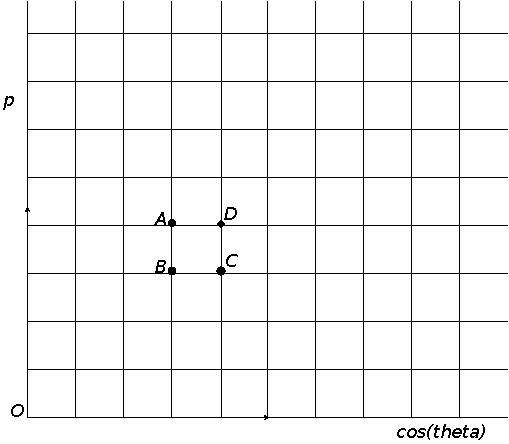
\includegraphics[width=0.6\textwidth]{chap4simul/Figures/kineGrid_steg.jpg} 
  %\leavevmode 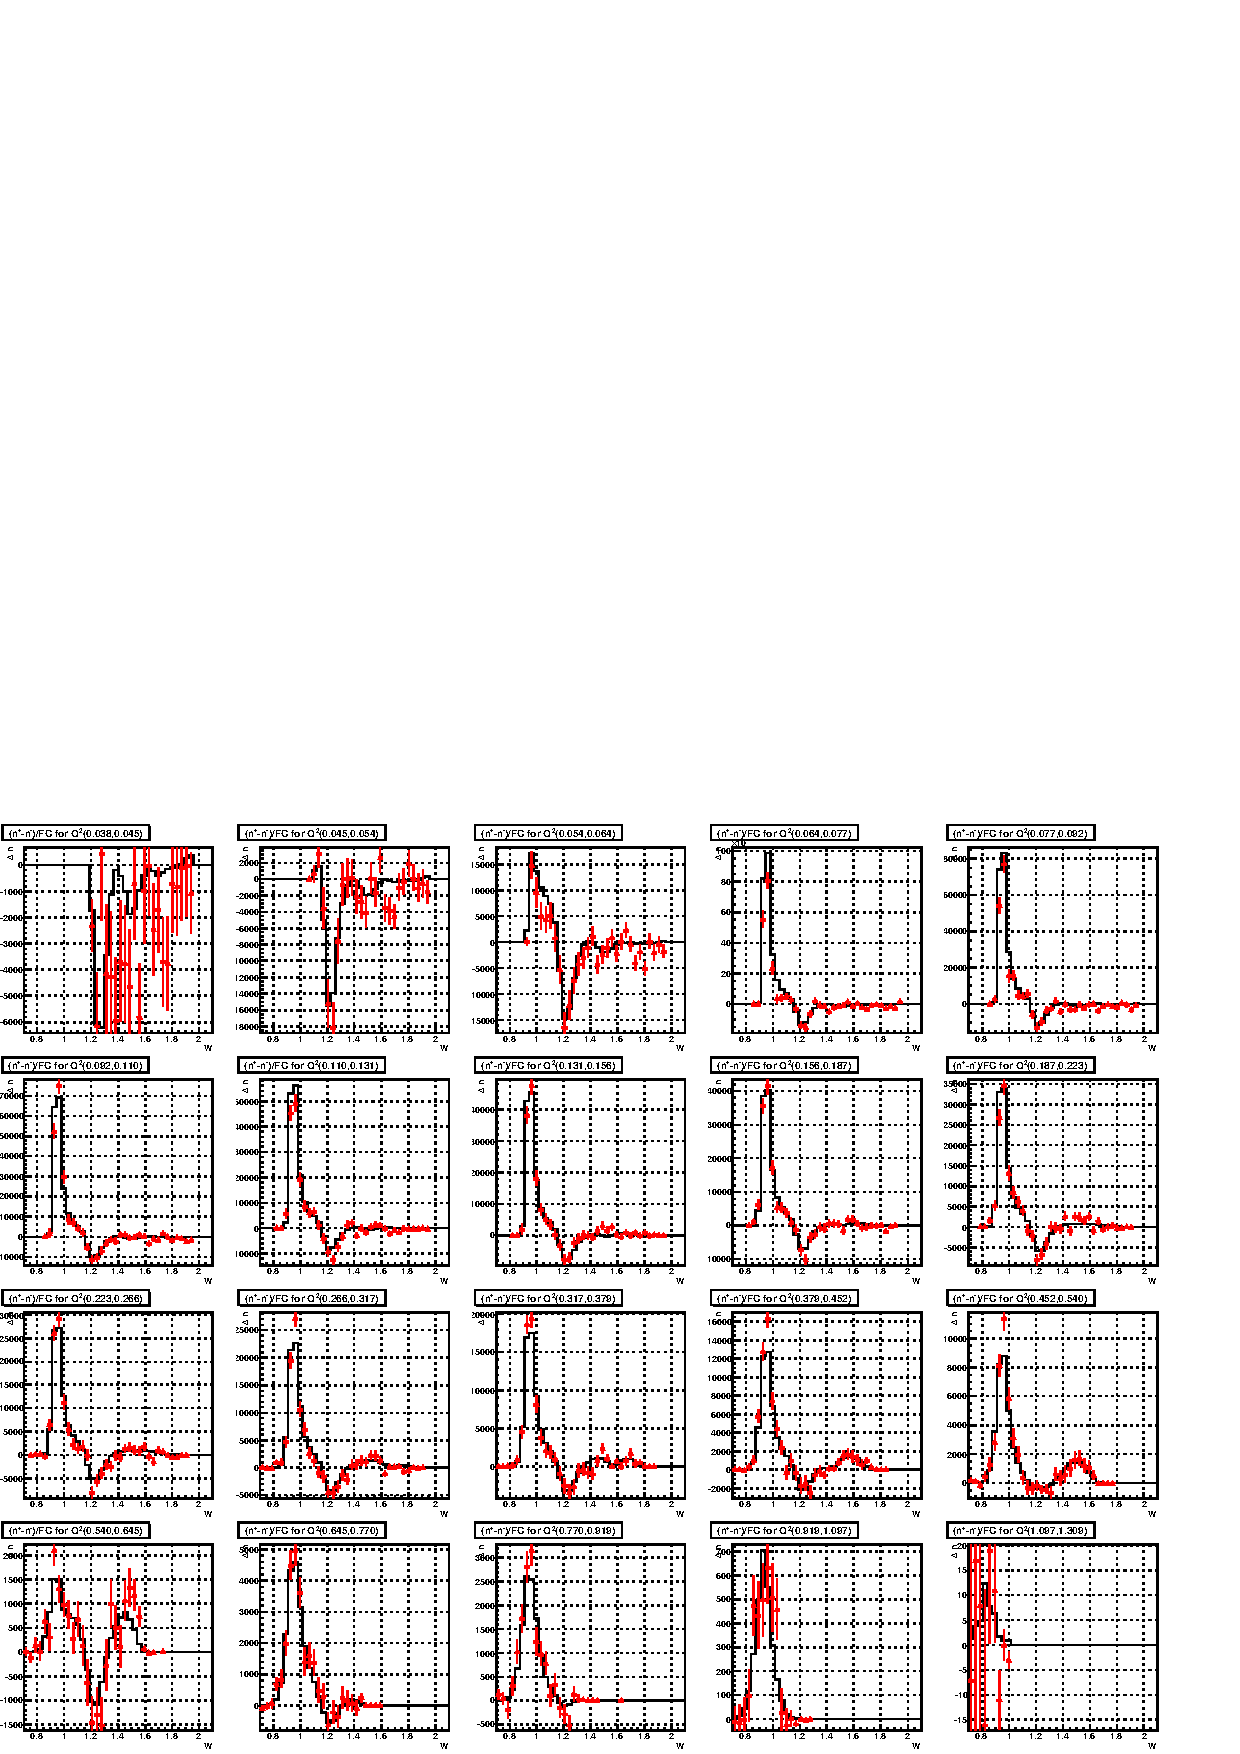
\includegraphics[width=1.0\textwidth]{figuresEG4/FigAnal/xsDifEb8VzD57HistC194S139.png}
  %\leavevmode 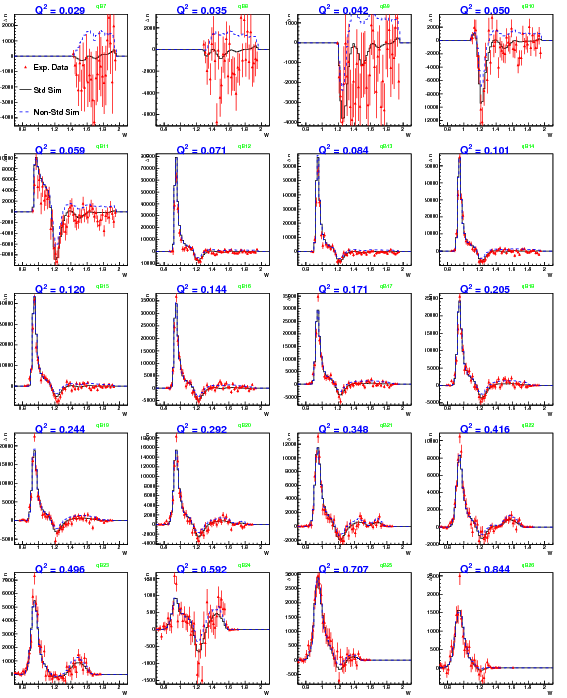
\includegraphics[width=1.0\textwidth]{figuresEG4/FigAnal/xsDiff_StdD57_nStdD62C194S139Eb8Wbins70N.png} 
  \leavevmode 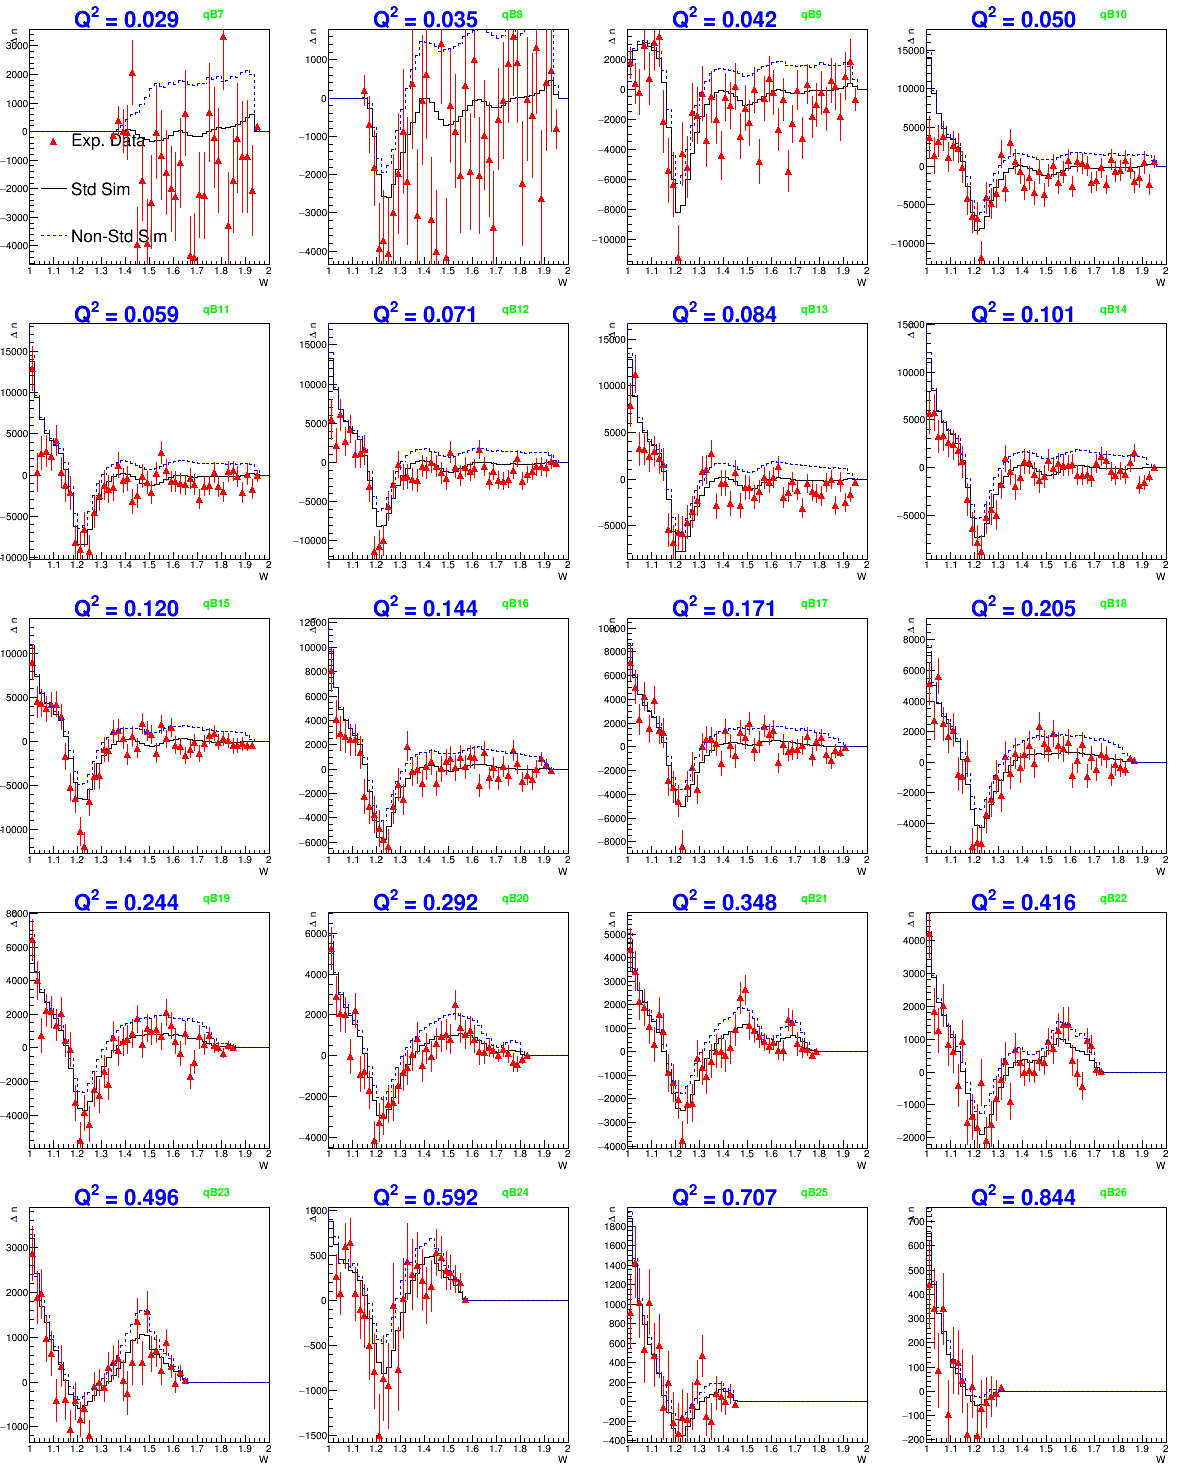
\includegraphics[width=0.97\textwidth]{figuresEG4/FigAnal/xsDiff_StdD79_nStdD80C71S181Eb8Wbins70NZmd.png}
  \caption[Count differences (2.0 GeV)]{Comparison (in different \qsqs bins) of polarized count differences from 2.0 GeV experimental (red points with error bars) and two versions of normalized simulation data. The black continuous histograms are for ``standard'' simulation with values of $A_1$ set as given by the used model. The blue dotted histograms are for ``non-standard'' simulated data with $A_1$ changed to $A_1 + 0.1$. }
  \label{xsComp8}  %http://wwwold.jlab.org/Hall-B/secure/eg4/adhikari/Simulations/mod_osip_bost_4kpDoc/steg.html
\end{figure}



After this normalization, the ratios $(n^+ - n^-)/\Delta n(simul)$ in the quasi-elastic region for all \qsqs %the momentum 
bins were calculated and plotted versus \qsqs as well as \ths %(which were somewhat similar to \ref{D2SvQ7qe}, \ref{D2SvTh7qe}, \ref{D2SvQ8qe}, and \ref{D2SvTh8qe} 
(see Figs. \ref{D2SvQ7qe} - \ref{D2SvTh8qe})
along with the corresponding statistical errors as given by $\sqrt{(n^+ + n^-)}/\Delta n(simul)$. As the figures show, the ratio in the quasi-elastic region drops %was observed to drop 
off rapidly at small \qsq. The fall-off is likely due to CC inefficiencies for very high momenta and very forward angles. Also, our simple cross section model for the deuteron is less accurate at low \qsq.  Figs. \ref{D2SvQ7del} - \ref{D2SvTh8del} show that the $\Delta$-resonance region does not suffer from similar problems %. %show such problems.
as the Delta model is quite reliable too (just like QE model).

%One last normalization was done again, with the nomalization factor obtained this time 
The final normalization was obtained by calculating the error weighted average $SF_{average}$ of above ratios in the quasi-elastic region%\footnote{The average was calculated using only those \qsqs bins which had ratios reasonably stable and closer to the expected value of 1.0. In the case of 1.337 GeV beam energy, the ratios from the first ten \qsqs bins as well as those with ratios greater than 2.5 were discared, and for the case of 1.993 GeV, those from the first thirteen bins as well as those that were greater than 2.0 were discarded from the average calculation.} 
. %and then multiplying the $\Delta n(simul)$. 
The average was calculated using only those \qsqs bins which had ratios reasonably stable and closer to each other. %the expected value of 1.0. 
Because, the ratios are reasonably stable only above $Q^2\approx 0.045$ GeV$^2$ and $Q^2 \approx 0.09$ GeV$^2$ in the 1.337 and 2.0 GeV data sets respectively (as can be seen from Figs. \ref{D2SvQ7qe} and \ref{D2SvQ8qe}), only those \qsqs bins above these two limits were used in calculating the weighted average of these ratios. In addition, even above those two limits, some of those which had too large ratios - greater than 2.0 (or 2.5) for 1.337 (or 2.0) GeV data set-  were not used in the weighted average. However, it should be noted that the bins not used in the average ratio calculations were not entirely discarded from the final analysis. Only those below $Q^2=0.02$ GeV$^2$ were completely thrown out from the final analysis because they did not cover the resonance (particularly the $\Delta$) region very well.
%In the case of 1.337 GeV beam energy, the ratios from the first ten \qsqs bins as well as those with ratios greater than 2.5 were not used, and for the case of 1.993 GeV, those from the first thirteen bins as well as those that were greater than 2.0 were not used in the average calculation. 
The resulting simulated data in the form of count differences $\Delta n$ in various \qsqs bins are %have been %SEK
shown in Figs. \ref{xsComp7} and \ref{xsComp8} along with the corresponding experimental data. %The corresponding plots of ratios vs \qsqs and \th in the quasi-elastic region as well as in the region encompassing the $\Delta$-resonance have been shown in figures \ref{D2SvQ7qe}, \ref{D2SvTh7qe}, \ref{D2SvQ8qe}, and \ref{D2SvTh8qe}. %SEK

A complete systematic error analysis was done to study the effect of the overall scaling factor $SF$ %$SF=SF_{20}\times SF_{average}$ 
on the extracted $g_1$ (see below) and to estimate its statistical (due to the number of counts) and systematic (due to model uncertainties and backgrounds) error. 

\begin{comment} %11/27/13:  ========= SEK: repetitive. Results for Chi-sq? either expand or leave out.
Fortunately, this did not require re-running the simulation!
In practice, one will determine this cross normalization factor %(kp: after above preliminary normalization)
 for each of the standard bins in $Q^2$ separately, including its statistical error, which is simply equal to 
\begin{equation}
\label{errSF}
\sigma_{SF} = \frac{\sqrt{n^+ + n^-}}{\Delta n(simul)} .
\end{equation}
A simple statistical analysis then gives the weighted mean of the results from all $Q^2$ bins, the corresponding standard deviation of the mean, and the $\chi^2$ which indicates whether the simulation describes the data reasonably accurate. %\textbf{\textcolor{red}{Should I list these numbers?.}} %remember the std. deviation and the Chi-sq per d.o.f that I calculated running compClasSimPolUnpol2.C
\end{comment}
%GetNormalizeSimXsDiffHistos(..) in extractStrFnG1.C used to get both standard and all-non-standard (including those for syst. errors) sim. histos
%In this function, the (first) normalization of p & n data w.r.t. their XS-map areas and #of sim. files (or # of events) is done.

% (Second) Normalization of sim. w.r.t. the CLAS data is done in NormalizeBothSimDataWrtExpData(..) of extractStrFnG1.C

%Once the 2nd normalization is done, we're ready to extract g1 and/or A1*F1



%  ==================        First the 1.3 GeV data


%The scale sizes below are hit and trial numbers chosen to make the figures as big as possible while putting them together
\begin{figure}[H] %[ht]
\centering
\subfigure[Data/Sim ratio vs $Q^{2}$ in 1.3 GeV quasi-elastic data.]{
%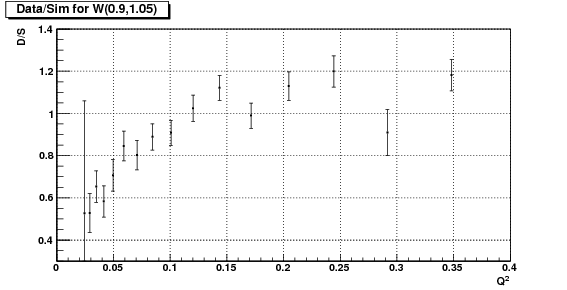
\includegraphics[scale=0.35]{figuresEG4/FigAnal/ratioVsQ2_QeData2simXsDifEb7VzD57HistC194S139.png} 
%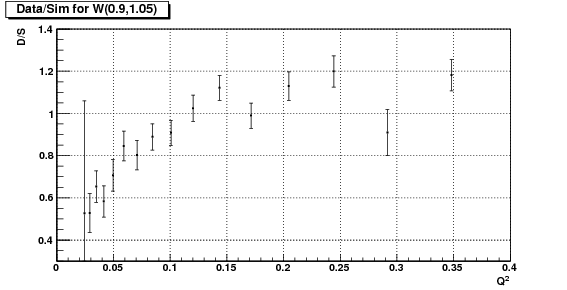
\includegraphics[scale=0.8]{figuresEG4/FigAnal/ratioVsQ2_QeData2simXsDifEb7VzD57HistC194S139.png} 
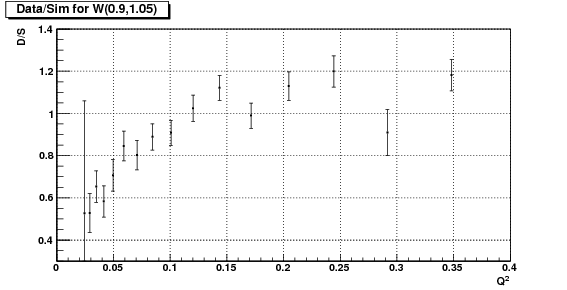
\includegraphics[scale=0.75]{figuresEG4/FigAnal/ratioVsQ2_QeData2simXsDifEb7VzD57HistC194S139} 
\label{D2SvQ7qe}
}\\
\subfigure[Data/Sim ratio vs $Q^{2}$ in $\Delta$-resonance region of 1.3 GeV data.]{
%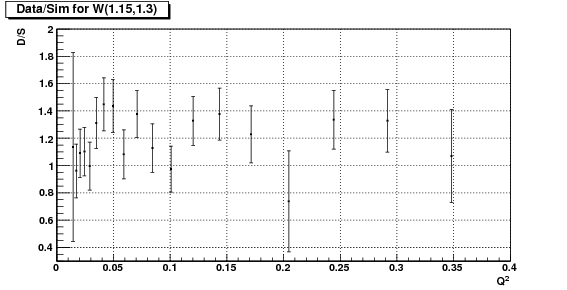
\includegraphics[scale=0.8]{figuresEG4/FigAnal/ratioVsQ2_DeltaData2simXsDifEb7VzD57HistC194S139.png} 
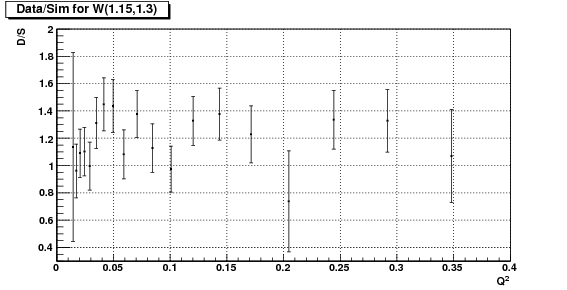
\includegraphics[scale=0.75]{figuresEG4/FigAnal/ratioVsQ2_DeltaData2simXsDifEb7VzD57HistC194S139} 
\label{D2SvQ7del}
}
\caption[Data to simulation ratios vs \qsq.]{\qsqs dependence of ratios of 1.3 GeV data and simulation in the quasi-elastic and $\Delta$-resonance regions.}
\label{D2SvQ7} %Effect of Dc-smear
\end{figure}




\begin{figure}[H] %[ht]
\centering
\subfigure[Data/Sim ratio vs $\theta$ in 1.3 GeV quasi-elastic data.]{
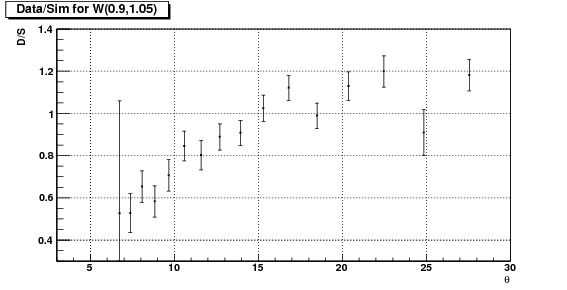
\includegraphics[scale=0.8]{figuresEG4/FigAnal/ratioVsTh_QeData2simXsDifEb7VzD57HistC194S139} 
\label{D2SvTh7qe}
}\\
\subfigure[Data/Sim ratio vs $\theta$ in $\Delta$-resonance region of 1.3 GeV data.]{
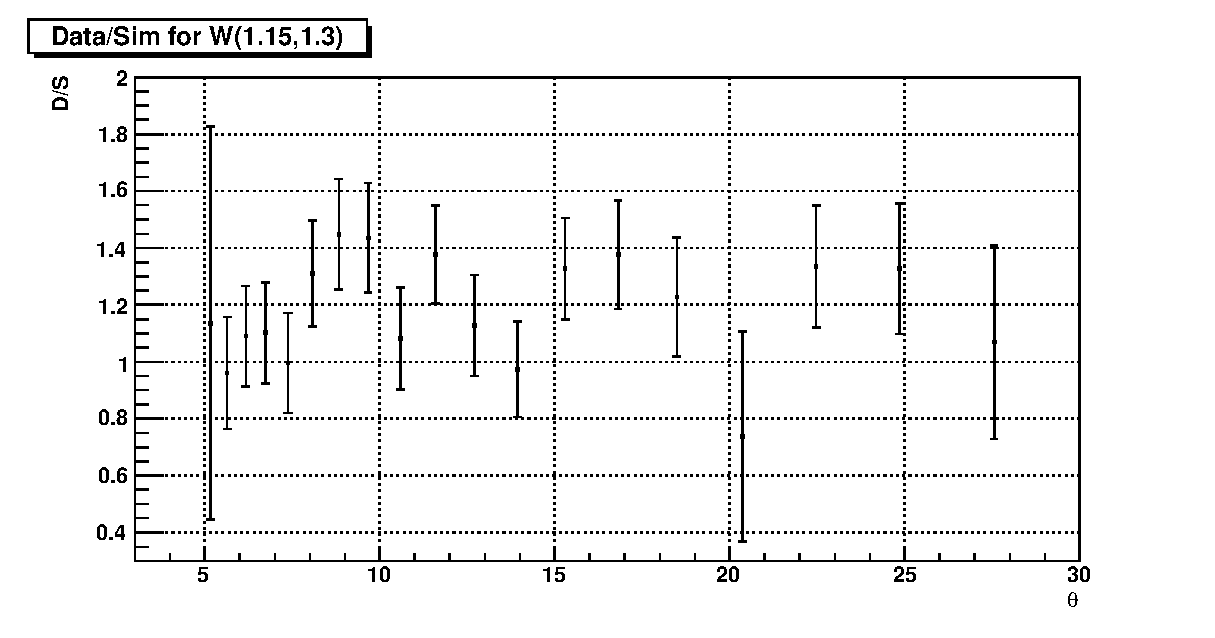
\includegraphics[scale=0.8]{figuresEG4/FigAnal/ratioVsTh_DeltaData2simXsDifEb7VzD57HistC194S139} 
\label{D2SvTh7del}
}
\caption[Data to simulation ratios vs \th]{The same data as in Fig. \ref{D2SvQ7}, but plotted versus average scattering angle (\thns). Here we can see that the data for $\theta > 10^{circ}$ reasonably stable with $\pm 10\%$ fluctuation (which will be taken into account while calculating the systematic uncertainty later.} %SEK comment
\label{D2SvTh7} %Effect of Dc-smear
\end{figure}


% =====================          Now 2.0 GeV data


\begin{figure}[H] %[ht]
\centering
\subfigure[Data/Sim ratio vs $Q^{2}$ in 2.0 GeV quasi-elastic data.]{
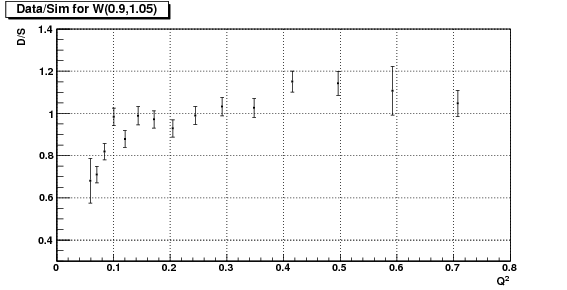
\includegraphics[scale=0.8]{figuresEG4/FigAnal/ratioVsQ2_QeData2simXsDifEb8VzD57HistC194S139} 
\label{D2SvQ8qe}
}\\
\subfigure[Data/Sim ratio vs $Q^{2}$ in $\Delta$-resonance region of 2.0 GeV data.]{
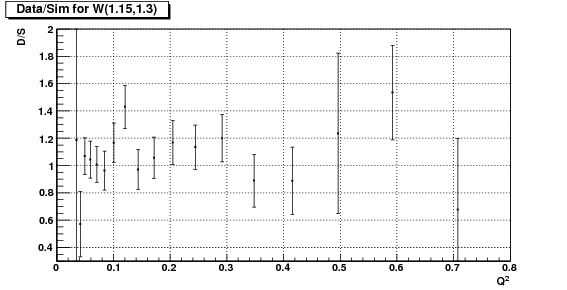
\includegraphics[scale=0.8]{figuresEG4/FigAnal/ratioVsQ2_DeltaData2simXsDifEb8VzD57HistC194S139} 
\label{D2SvQ8del}
}
\caption[Data to simulation ratios vs \qsqs (2.0 GeV)]{\qsqs dependence of ratios of 2.0 GeV data and simulation in the quasi-elastic and $\Delta$-resonance regions.}
\label{D2SvQ8} %Effect of Dc-smear
\end{figure}


\begin{figure}[H] %[ht]
\centering
\subfigure[Data/Sim ratio vs $\theta$ in 2.0 GeV quasi-elastic data.]{
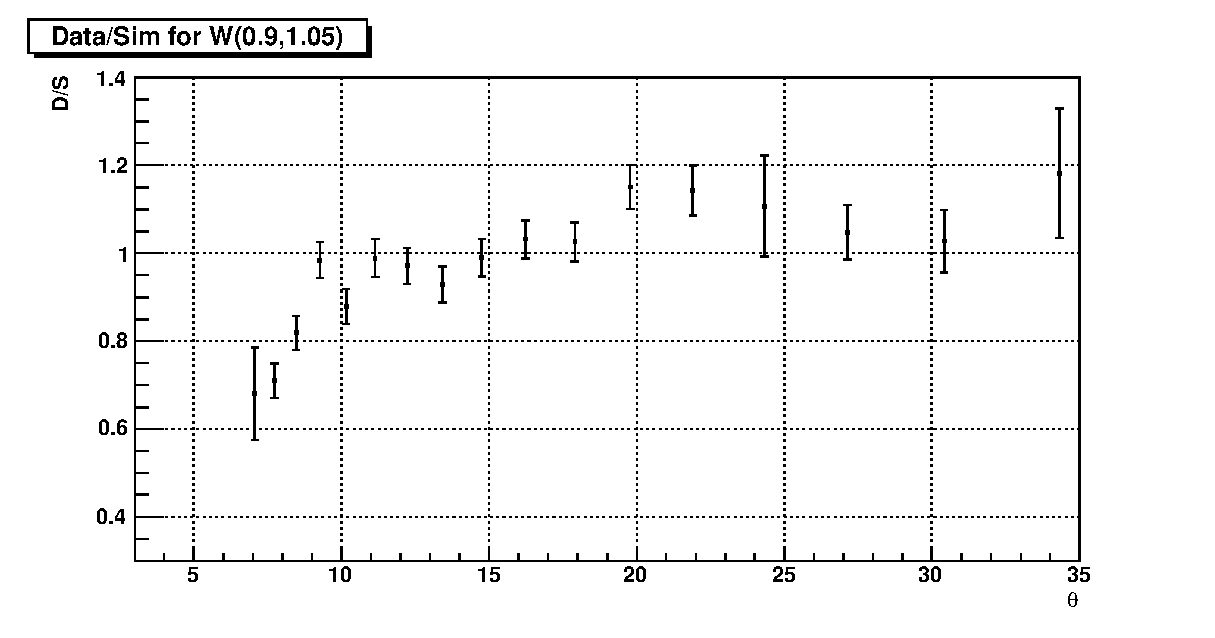
\includegraphics[scale=0.8]{figuresEG4/FigAnal/ratioVsTh_QeData2simXsDifEb8VzD57HistC194S139} 
\label{D2SvTh8qe}
}\\
\subfigure[Data/Sim ratio vs $\theta$ in $\Delta$-resonance region of 2.0 GeV data.]{
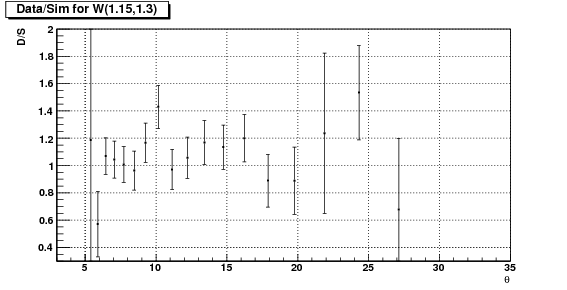
\includegraphics[scale=0.8]{figuresEG4/FigAnal/ratioVsTh_DeltaData2simXsDifEb8VzD57HistC194S139} 
\label{D2SvTh8del}
}
\caption[Data to simulation ratios vs \th (2.0 GeV)]{The same data as in Fig. \ref{D2SvQ8}, but plotted versus average scattering angle (\thns). Here we can see that the data for $\theta > 10^{circ}$ reasonably stable with $\pm 10\%$ fluctuation (which will be taken into account while calculating the systematic uncertainty later.} %{\th dependence of ratios of 2.0 GeV data and simulation in the quasi-elastic and $\Delta$-resonance regions.}
\label{D2SvTh8} %Effect of Dc-smear
\end{figure}



